\documentclass{article}
\usepackage{indentfirst}
\usepackage[margin=3cm]{geometry}
\usepackage{listings}
\usepackage{xcolor}
\usepackage{graphicx}
\graphicspath{ {~/dox/cs/pythogorean-magic} }

\definecolor{codegreen}{rgb}{0,0.6,0}
\definecolor{codegray}{rgb}{0.5,0.5,0.5}
\definecolor{codepurple}{rgb}{0.58,0,0.82}
\definecolor{backcolour}{rgb}{0.95,0.95,0.92}

\lstdefinestyle{mystyle}{
    commentstyle=\color{codegreen},
    keywordstyle=\color{magenta},
    numberstyle=\tiny\color{codegray},
    stringstyle=\color{codepurple},
    basicstyle=\ttfamily\footnotesize,
    breakatwhitespace=false,
    breaklines=true,
    captionpos=b,
    keepspaces=true,
    numbers=left,
    numbersep=5pt,
    showspaces=false,
    showstringspaces=false,
    showtabs=false,
    tabsize=2
}

\lstset{style=mystyle}

\begin{document}

\section{Analysis}
\begin{itemize}
    \item \textbf{The outline of the problem:} user inputs three sides of a
        triangle, the program identifies whether it is right angled and draws
        it.
    \item \textbf{Stakeholders:} the client is the Head of Mathematics at DLD
        College London.
    \item \textbf{Research:} how to use turtle graphics in python in order to
        draw a triangle.
    \item \textbf{Success criteria \& features:} the program will be successful
        if it will correctly identify a triangle, draw it, handle any input, be
        user friendly and intuitive to use, readable and well-documented (the
        code), follow the PEP-8 convention,  will not crash, contain severe
        bugs or cause any frustration to a user.
\end{itemize}

\section{Design}
\begin{itemize}
    \item Flow-chart:

\begin{figure}[h]
	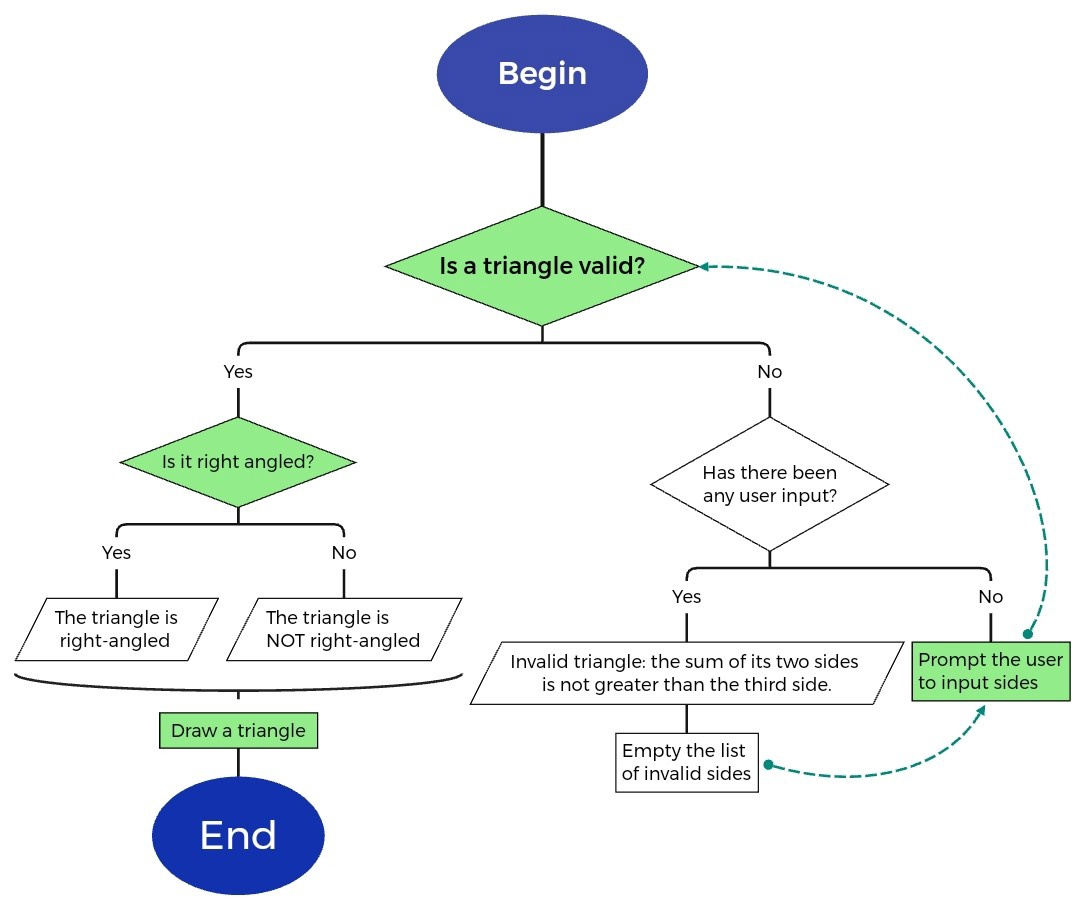
\includegraphics[scale=0.35]{flow-chart.jpg}
	\centering
\end{figure}

    \item Rhomboids represent choices, parallelograms -- outputs, green
        background means function, rectangles are actions.

    \item The lengths entered by a user will be stored in a list as strings,
        which after all the validation checks will be converted into integers
        and sorted in the descending order.

    \item The function which prompts the user to input sides includes another
        function that determines whether the input is a positive integer.

    \item Test data:
\begin{itemize}
    \item 1, 1, 1 \textbf{[PASSED]}
    \item 3, 4, 5 \textbf{[PASSED]}
    \item 4, 3, 5 \textbf{[PASSED]}
    \item 5, 4, 3 \textbf{[PASSED]}
    \item 7, 9, 8 \textbf{[PASSED]}
    \item 8, 14, 8 \textbf{[PASSED]}
    \item 0 \textbf{[PASSED]}
    \item 1.5 \textbf{[PASSED]}
    \item -3 \textbf{[PASSED]}
    \item abc \textbf{[PASSED]}
    \item *\&\#@ \textbf{[PASSED]}
    \item $<$CR$>$ \textbf{[PASSED]}
    \item 1, 2, 999 \textbf{[PASSED]}
    \item 300000, 400000, 500000 \textbf{[PASSED]}
    \item 100, 99, 98 \textbf{[PASSED]}
    \item 1, 100, 1 \textbf{[PASSED]}
\end{itemize}
\end{itemize}

\section{Development}
\begin{itemize}
    \item The program is well-documented with a sufficient use of comments and
        documentation strings for functions, so it is easy to understand and
        navigate.
    \item It is separated into smaller functions to ensure code re-usability
        and readability, therefore the entire logic of the program can be
        observed in the main function:
\begin{lstlisting}[language=Python]
import math
import turtle

def main():
    sides = []
    # Prompt the user to enter lengths until all the requirements are met.
    while not triangle_is_valid(sides):
        # Don't show the error message on the
        # first try (if the list is empty).
        if sides:
            sides.clear()
            print('Invalid triangle: the sum of its two sides '
                  'is not greater than the third side.')
        sides = input_sides(sides)

    if is_right_angled(sides):
        print(f'The triangle with sides {sides[0]}, '  # The use of f-strings.
              f'{sides[1]} and {sides[2]} IS right angled.')
    else:
        print(f'The triangle with sides {sides[0]}, '
              f'{sides[1]} and {sides[2]} is NOT right angled.')

    draw_triangle(sides)


if __name__ == '__main__':
    main()
\end{lstlisting}
\break
    \item The program starts with a loop that ensures that a correct input has
        been provided. It will continue prompting the user until numerous
        validation checks are passed:
\begin{lstlisting}[language=Python]
def input_sides(sides):
    """Get a valid input from the user and format it appropriately."""
    i = 0
    while i < 3:
        sides.append(input(f'Please enter the length of the #{i+1} side: '))
        if side_is_valid(sides[i]):
            i += 1
        else:
            sides.pop()
    # Convert strings to integers.
    sides = [int(i) for i in sides]  # The use of list comprehension.
    sides.sort()
    return sides


def side_is_valid(side_len):
    """Check if the entered length is a positive integer."""
    # Check if it's an integer.
    try:  # The use of exception handling.
        int(side_len)
    except ValueError:
        print('The length must be an integer.')
        return False

    # Check if it's positive.
    if int(side_len) <= 0:
        print('The length must be positive.')
        return False
    else:
        return True


def triangle_is_valid(sides):
    """
    Check if the user has entered three
    lengths that meet the triangle inequality.
    """
    try:
        a = sides[0]
        b = sides[1]
        c = sides[2]
    except IndexError:
        return False

    # The triangle inequality.
    if a+b>c and a+c>b and b+c>a:
        return True
    else:
        return False
\end{lstlisting}

    \item Next, it is determined whether a triangle is right-angled or not:
\begin{lstlisting}[language=Python]
def is_right_angled(sides):
    """Check if the triangle is right angled or not."""
    short_cathetus = sides[0]
    long_cathetus = sides[1]
    hypotenuse = float(sides[2])  # math.sqrt returns float.
    # The Pythagorean theorem.
    if hypotenuse == math.sqrt(short_cathetus**2 + long_cathetus**2):
        return True
    else:
        return False
\end{lstlisting}

\item Lastly, the triangle is drawn. This function incorporates the law of
    cosines to find the angles and it automatically sets the scale based on the
    user's input, so that both big (i.e. 300, 400, 500) and small (i.e. 1, 1,
    1) triangles could be clearly visible:
\begin{lstlisting}[language=Python]
def draw_triangle(sides):
    """Draw a triangle."""  # The use of a documentation string.
    a = sides[0]
    b = sides[1]
    c = sides[2]
    # Use the law of cosines to find the angles.
    b_angle = math.degrees(math.acos((a**2 + b**2 - c**2) / (2*a*b)))
    c_angle = math.degrees(math.acos((b**2 + c**2 - a**2) / (2*b*c)))

    t = turtle.Turtle()
    # Set the scale based on the largest length.
    scale_factor = 10**len(str(c))
    turtle.setworldcoordinates(0, 0, scale_factor, scale_factor)
    # Set the speed of drawing to maximum.
    t.speed(10)

    # Draw side a.
    t.forward(a)
    t.left(180 - b_angle)
    # Draw side b.
    t.forward(b)
    t.left(180 - c_angle)
    # Draw side c.
    t.forward(c)

    turtle.done()
\end{lstlisting}

\end{itemize}

\section{Evaluation}
\begin{itemize}
    \item The program has successfully met all the criteria and features set in
        the Analysis section, and passed every test in the Design section.
    \item Potential maintenance problems could occur if something happens to
        the external libraries used or in case more users test the program on
        different devices. Since I am neither maintaining the libraries, nor
        have resources to conduct such a thorough testing, I am currently
        unable to prevent these potential issues.
    \item One of the limitations of the program is that while it has
        auto-scaling, it lacks user control. For instance, one might want to
        manually decrease the scale in real time or move/rotate the triangle in
        order to better inspect it. More details can be provided on the drawing
        and in the output (i.e. angles).  Moreover, a system of saving the
        results in a file (both drawing and parameters) may be implemented.
\end{itemize}
\end{document}
